Zum  Vergleich  mit  den  soeben  dimensionierten  PI-  und  PID-Reglern  sind
hier   noch  die   Resultate   der  Dimensionierung   mittels  unseres   Tools
gezeigt. Wie  zu erwarten  weisen die  mit  dem Tool  berechneten Werte  f\"ur
die  Faustformeln   keine  signifikanten  Abweichenungen  zu   den  Werten  in
Tabelle~\ref{tab:ff_results} auf.

Verwendet man  in den Berechnungen mittels  Phasengangmethode den Standardwert
f\"ur $\varphi_r$,  erh\"alt man Zahlen,  die ziemlich  nahe bei den  von Hand
berechneten Resultaten liegen. Wird jedoch von den Optimierungsm\"oglichkeiten
des   Tools  Gebrauch   gemacht,   \"andern  sich   die  Reglerparameter   und
das   Verhalten  des   zugeh\"origen   geschlossenen  Regelkreises   teilweise
betr\"achtlich.

Die        Zahlenwerte       sind        in       Tabelle~\ref{tab:allresults}
zusammengefasst,       einige       Plots        zum       Vergleich       der
Schrittantworten    der   zugeh\"origen    geschlossenen   Regelkreise    sind
in    den    Abbildungen~\ref{fig:comparisonPI015},~\ref{fig:comparisonPID015}
und~\ref{fig:comparisonPID002optimisations} zu sehen.

\begin{longtable}{p{85mm}rrrrr}
    \toprule

    %\multicolumn{3}{l}{\large{\textsc{Auftragsanalyse und Hintergrundinformationen}}} \\

    Berechnungsmethode
    &
    \multicolumn{2}{l}{PI-Regler}
    &
    \multicolumn{2}{l}{PID-T1-Regler}
    \\

    &
    $T_n$
    &
    $K_p$
    &
    $T_n$
    &
    $T_v$
    &
    $K_p$
    \\

    \midrule

    \endhead
    \endfoot
    \endlastfoot

    % CONTENT HERE ---------------------------------------------------------- %

    \pbox{84mm}{Chiens, Hrones, Reswick (manuell) \\ \small{\textbf{(0\% \"Uberschwingen)}}~\cite{ref:chiens_tsn},~\cite{ref:chiens_wiki}}
    &
    $\SI{10.68}{\second}$
    &
    $1.42$
    &
    $\SI{8.9}{\second}$
    &
    $\SI{0.55}{\second}$
    &
    $2.43$
    \\

    \addlinespace[0.5em]

    \pbox{84mm}{Chiens, Hrones, Reswick (Software) \\ \small{\textbf{(0\% \"Uberschwingen)}}}
    &
    $\SI{10.68}{\second}$
    &
    $1.42$
    &
    $\SI{8.9}{\second}$
    &
    $\SI{0.55}{\second}$
    &
    $2.43$
    \\

    \addlinespace[0.5em]

    \pbox{84mm}{Chiens, Hrones, Reswick (manuell) \\ \small{\textbf{(20\% \"Uberschwingen)}}~\cite{ref:chiens_tsn},~\cite{ref:chiens_wiki}}
    &
    $\SI{8.9}{\second}$
    &
    $2.43$
    &
    $\SI{12.02}{\second}$
    &
    $\SI{0.52}{\second}$
    &
    $3.84$
    \\

    \addlinespace[0.5em]

    \pbox{84mm}{Chiens, Hrones, Reswick (Software) \\ \small{\textbf{(20\% \"Uberschwingen)}}}
    &
    $\SI{8.9}{\second}$
    &
    $2.43$
    &
    $\SI{12.02}{\second}$
    &
    $\SI{0.517}{\second}$
    &
    $3.84$
    \\

    \addlinespace[0.5em]

    Oppelt (manuell)~\cite{ref:op_ros_zieg}
    &
    $\SI{3.3}{\second}$
    &
    $3.24$
    &
    $\SI{2.2}{\second}$
    &
    $\SI{0.46}{\second}$
    &
    $4.85$
    \\

    \addlinespace[0.5em]

    Oppelt (Software)
    &
    $\SI{3.3}{\second}$
    &
    $3.24$
    &
    $\SI{2.20}{\second}$
    &
    $\SI{0.462}{\second}$
    &
    $4.85$
    \\

    \addlinespace[0.5em]

    Rosenberg (manuell)~\cite{ref:op_ros_zieg}
    &
    $\SI{3.63}{\second}$
    &
    $3.68$
    &
    $\SI{2.2}{\second}$
    &
    $\SI{0.50}{\second}$
    &
    $4.85$
    \\

    \addlinespace[0.5em]

    Rosenberg (Software)
    &
    $\SI{3.63}{\second}$
    &
    $3.68$
    &
    $\SI{2.20}{\second}$
    &
    $\SI{0.495}{\second}$
    &
    $4.85$
    \\

    \addlinespace[0.5em]

    \pbox{84mm}{Phasengangmethode (manuell) \\ \small{\textbf{(16.3\% \"Uberschwingen)}} \\}
    &
    $\SI{3.29}{\second}$
    &
    $0.52$
    &
    $\SI{5.37}{\second}$
    &
    $\SI{0.41}{\second}$
    &
    $1.83$
    \\

    \addlinespace[0.5em]

    \pbox{84mm}{Phasengangmethode (Software) \\ \small{\textbf{(15\% \"Uberschwingen)}} \\}
    &
    $\SI{3.29}{\second}$
    &
    $0.47$
    &
    $\SI{5.74}{\second}$
    &
    $\SI{0.35}{\second}$
    &
    $1.78$
    \\

    \addlinespace[0.5em]

    \pbox{84mm}{Phasengangmethode (Software, $\varphi_r$ Standard) \\ \small{\textbf{(2\% \"Uberschwingen)}} \\}
    &
    $\SI{3.29}{\second}$
    &
    $0.17$
    &
    $\SI{5.74}{\second}$
    &
    $\SI{0.35}{\second}$
    &
    $0.76$
    \\

    \addlinespace[0.5em]

    \pbox{84mm}{Phasengangmethode (Software, Optimierungen positiv) \\ \small{\textbf{(2\% \"Uberschwingen)}} \\}
    &
    $\SI{7.50}{\second}$
    &
    $1.05$
    &
    $\SI{13.02}{\second}$
    &
    $\SI{0.636}{\second}$
    &
    $2.70$
    \\

    \addlinespace[0.5em]

    \pbox{84mm}{Phasengangmethode (Software, Optimierungen negativ) \\ \small{\textbf{(2\% \"Uberschwingen)}} \\}
    &
    $\SI{1.62}{\second}$
    &
    $0.058$
    &
    $\SI{5.74}{\second}$
    &
    $\SI{0.35}{\second}$
    &
    $0.76$
    \\

    \addlinespace[0.5em]


    \bottomrule
    \caption{%
        Zusammenfassung   und  Vergleich   der   mit  verschiedenen   Methoden
        berechneten Regelparameter.
    }
\label{tab:allresults}
\end{longtable}


\begin{minipage}[c][][b]{.75\textwidth}
    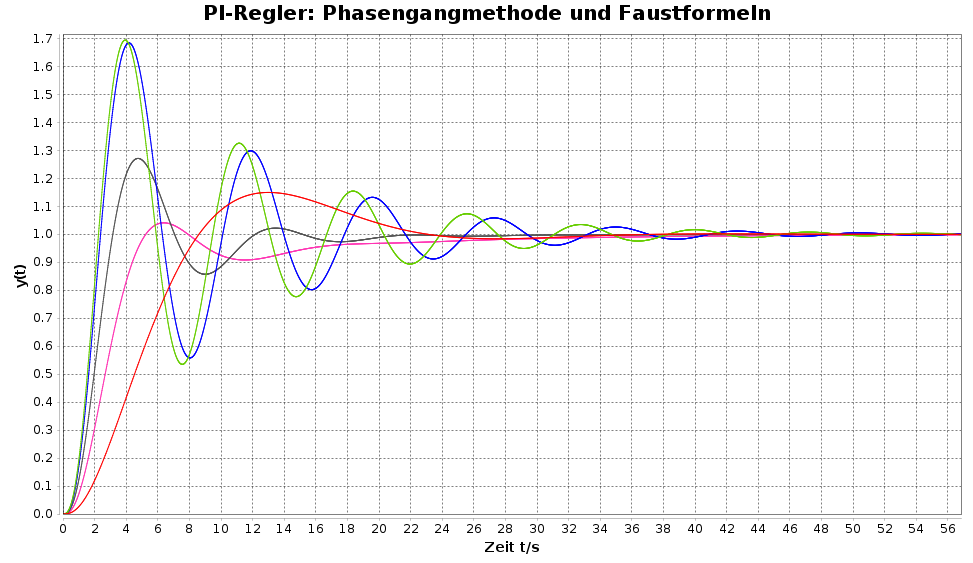
\includegraphics[width=\textwidth]{images/comparisonPI015.png}
\end{minipage}
\begin{minipage}[c][][b]{.22\textwidth}
    \captionof{figure}{%
        Schrittantworten    des   geschlossenen    Regelkreises (PI-Regler):
        \textbf{Pink}: Chiens, Hrones, Reswick (0\% \"Uberschwingen),
        \textbf{dunkelgrau}: Chiens, Hrones, Reswick (20\% \"Uberschwingen),
        \textbf{blau}: Oppelt,
        \textbf{gr\"un}: Rosenberg,
        \textbf{rot}: Phasengangmethode.
    }
    \label{fig:comparisonPI015}
\end{minipage}

\begin{minipage}[c][][b]{.75\textwidth}
    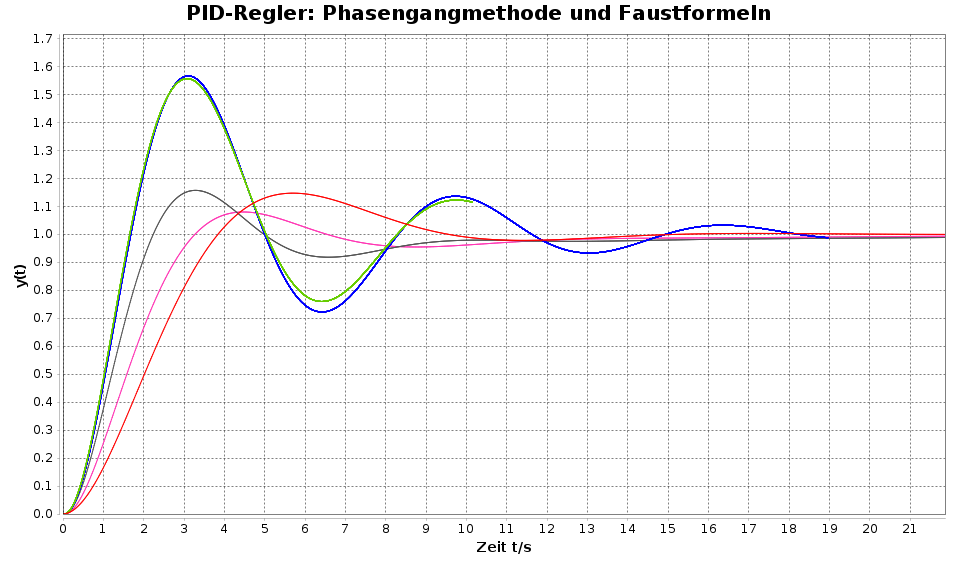
\includegraphics[width=\textwidth]{images/comparisonPID015.png}
\end{minipage}
\begin{minipage}[c][][b]{.22\textwidth}
    \captionof{figure}{%
        Schrittantworten    des   geschlossenen    Regelkreises (PID-Regler):
        \textbf{Pink}: Chiens, Hrones, Reswick (0\% \"Uberschwingen),
        \textbf{dunkelgrau}: Chiens, Hrones, Reswick (20\% \"Uberschwingen),
        \textbf{blau}: Oppelt,
        \textbf{gr\"un}: Rosenberg,
        \textbf{rot}: Phasengangmethode.
    }
    \label{fig:comparisonPID015}
\end{minipage}

\begin{minipage}[c][][b]{.75\textwidth}
    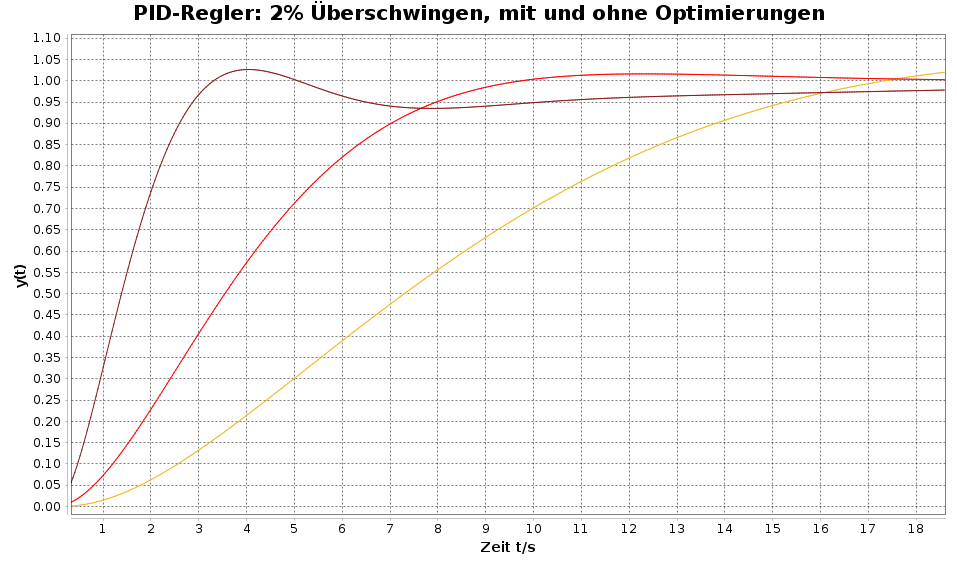
\includegraphics[width=\textwidth]{images/comparisonPID002optimisations.png}
\end{minipage}
\begin{minipage}[c][][b]{.22\textwidth}
    \captionof{figure}{%
        Schrittantworten    des   geschlossenen    Regelkreises (PID-Regler),
        \"Uberschwingen auf 2\% begrenzt, mit Optimierungen:
        \textbf{rot}: Phasengangmethode (Standardwerte),
        \textbf{braun}: Phasengangmethode (positiv optimiert),
        \textbf{gelb}: Phasengangmethode (negative optimiert).
    }
    \label{fig:comparisonPID002optimisations}
\end{minipage}
